\documentclass[journal]{IEEEtran}


\usepackage[subpreambles=false]{standalone}
\usepackage{import}
\usepackage{tikz}
\usetikzlibrary{shapes,shapes.geometric,shapes.multipart}\usetikzlibrary{arrows.meta}
\usepackage{tabularx}
\usepackage{adjustbox}
\usepackage{blindtext}

\let\oldref\ref
\renewcommand{\ref}[1]{(\oldref{#1})}

\usepackage[backend=biber, sorting=none, style=numeric-comp]{biblatex}
\addbibresource{../sections/references.bib}

\begin{document}

\title{Making~Analysis~of~Power~Systems \\Scalable~through~Distributed~Computing}


\author{Aryan~Ritwajeet~Jha \\ \IEEEmembership{Pursuing~PhD~ECE~(Power Systems) \\ Department~of~Electrical~Engineering~and~Computer~Science \\ ~Washington~State~University,~Pullman}
        % <-this % stops a space
}

% The paper headers
\markboth{Fall 2022~EE~521~Analysis~of~Power~Systems}%
{Aryan Ritwajeet Jha's Final Paper}

\maketitle

\begin{abstract}
Distributed Computing is among the methods/concepts used to speed-up computation or ease computation overload in systems, which are typically analyzed all at once. Distributed Computing is an effective solution for Power Distribution Systems, which are typically highly heterogeneous and hard to solve for via conventional `centralized algorithms'. Distributed Computation is also an attractive method to ensure privacy of key state variables among multiple parties, such as TSOs, which normally require to cooperate with each other as being part of the same grid, but would want to exchange only as much data as would be essential for running and maintaining the power system. Lastly Distributed Computing is also highly desirable for increasing the bulk of sampled data, which ensures a more reliable state estimation of the power system. In this paper first the need for Distributed Computing is motivated, then some clarification is done on the term in order to remove any ambiguities from some other common usages for the same term. Lastly, through gists of other scientific literature on the topic, the implementation and effectiveness of Distributed Computing is highlighted.
\end{abstract}

\begin{IEEEkeywords}
Distributed~Computing, Parallel~Processing, Sparse~Algorithms, State~Estimation, Power~Flow~Analysis, Optimal~Power~Flow, Power~Distribution~Systems
\end{IEEEkeywords}

\IEEEpeerreviewmaketitle

\section{Introduction}

\IEEEPARstart{D}{istributed} Computing is the process of dividing a system (problem) into several smaller sub-systems (sub-problems), and instead of analyzing the whole system at once via a single `centralized' algorithm, each sub-system is separately analyzed, and then the respective analyses are coordinated together in order to possibly arrive at a `solution' which satisfies the whole system. There are several algorithms devised to approach the problem, common ones employed being Alternating Direction of Multipliers Method (ADMM) algorithm and the ALADIN algorithm \cite{aladinAlgorithmPaper}. However the problems can also be solved for using the usual centralized approaches such as Dual Problem formulation, Lagrangian Min-Maxing, Simplex Algorithms, Semi-Definite Programming, Second-Order Conic Programming Relaxation, Interior Point Methods, etc.

One caveat to the usage of the term `Distributed Computing' is the high number of different usages for the same across literature and scientific and engineering division. Such literature, while often refer to very similar things, such as Parallel Processing, Sparse Algorithms, Single-Instruction-Multi-Data processing, Advanced Signal Processing Algorithms using the same term, the difference could be confusing to the readers. So this paper also clarifies the specific usage of the term relevant to the paper. 

Next this paper also highlights the importance of Distributed Computing via some examples involving computational overhead, ill-behaved systems which are hard to solve for, privacy conflicts between different entities, both at the same level of a hierarchy and different level of a hierarchy.

Lastly this paper highlights specific examples where the usage of Distributed Computing is not only attractive but in fact necessary, as certain large but highly ill-behaved systems cannot be solved for using conventional centralized algorithms, in which case distributed computational algorithms come to the rescue.

The rest of the paper is as follows: Section \ref{motivation} provides a brief motivation for pursuing this topic for the paper as part of the course. Section \ref{practice} describes the practical implementation of each method. Lastly, Section \ref{comparison} compares the advantages and disadvantages of these methods.

\section{Motivation}
Prior to coming to Washington State University, I've always worked in Power System Control and Stability, which typically is employed on well-behaved Transmission Systems. They are called well-behaved due to the following reasons:
\begin{enumerate}
	\item Low R/X Ratio
	\item Dominant $Y_{Bus}$ and Jacobians
	\item Stable $LU$ matrices
	\item Balanced Three-Phase Systems
\end{enumerate}

After joining WSU, I was assigned to read on Power Distribution Systems, which are quite the opposite of Transmission Systems, in the way that:
\begin{enumerate}
	\item They have a high R/X Ratio.
	\item They have ill-behaved $Y_{Buses}$ and Jacobians
	\item $LU$ Matrices are susceptible to `breaking' mid-iteration
	\item Typically unbalanced three-phase systems
	\item Shorter distribution lines lead to non-diagonally-dominant matrices.
	\item Instead of stable meshed networks, the distribution lines are basically radial networks, generally with a single point of power source.
	\item Highly non-homogeneous loading schemes for every feeder bus, and many feeder buses for every substation.
\end{enumerate}
\label{motivation}
 
\section{Distributed Computing: Why you should do it?}

\cite{fastNRPFBasedOnSparseTechniquesAndParallelProcessing} was used to describe a case when the usage of distributed computing, albeit not, as the actual methods used included parallel processing via multi-core CPUs and Single-Instruction-Multi-Data (SMID) chips in conjunction with Sparse Techniques such as Compressed Row Storage (CSR). It can be called a good starting point for showing the scalability and speed of Distributed Computing, as it was seen in its results that it could achieve a $+150\%$ increment on the speed for processing large ($30000$ bus) synthetic systems over MATPOWER's \textit{runpf} module, which itself is known to be very fast.

Paper \cite{aladinAlgorithmPaper} highlights the need for privacy among different members of the power grid such as TSOs and why sharing all of the state variables of a sub-system with all other sub-systems is NOT a necessity when solving for a bigger system.

Paper \cite{gomez_exposito_multilevelStateEstimationParadigm} highlights how distributed computing enables the efficient and relevant grassroots level collection of data at a large level, significant enough to ensure that the data is:
\begin{itemize}
	\item \textbf{Redundant}: Redundancy is the concept of having more measurements ($m$) than the number of state variables we with to compute ($n$). If we have more (than one) measurements for a single state variable, say the bus voltage at a particular bus or the line current at a particular branch, chances are that even if one of the devices reporting the state variable value is an errant one, i.e. it is reporting incorrect values, the consensus measurement obtained by a simple majority polling of the measurements of all the devices measuring the same state variable will filter out all the bad data, leading to accurate, reliable and meaningful data for the state variable, which is both convenient for reporting to a higher level (such a TSO Transmission System Operator reporting to a RSO Regional System Operator) or even for interacting with other subsystems at the same level (such as a substation exchanging border state variables with neighbouring state variables).
	\item Easier to process: It makes sense for the data for a secondary level feeder to be processed at the feeder level itself, rather than delegating it to the TSO level and then having it processed there. This is because the TSO has no way of customizing the assumptions of the load demand and generation profile of a particular feeder, let alone account for the fact that the feeder's data is actually not even balanced in the tree phases. Since every feeder has its unique individual power profile, the data processing is best done via remote devices such as PMUs Phasor Measurement Units and IEDs Intelligent Electronic Devices, so that they are processed before sending to the next level. This eases the computational overload on the TSO by a hundred times. \cite{gomez_exposito_multilevelStateEstimationParadigm}
\end{itemize}

Then paper \cite{aladinAlgorithmPaper} also highlights the need of privacy among different constituents on the same power grid. For example if a German TSO and a Dutch TSO are interconnected and would require to interact via exchange enough inner data for a smooth functioning of the grid, it would be in each's best interest to not reveal key strategic generation and distribution data with each other.

This highlights another key merit of Distributed Computing:
\begin{itemize}
	\item Privacy: In order to maintain data privacy among different member of the same systems, the authors of \cite{aladinAlgorithmPaper} suggested a paradigm in which the subsystems only exchange the border state variables fully, while only providing a general (but reasonably accurate) depiction of the interior state variables, via something like a probability distribution function. This way the constituent subsystems do not have to compromise on their privacy while still ensuring that the systems is analyzed in a computationally efficient, safe and secure manner.
\end{itemize} 

\section{Distributed Computing: Why you must do it?}
\label{comparison}
An advantage of the distributed computing based method over the other methods is that it provides the easiest way to `clean' the live data of any noise via simple signal processing techniques, including windowing and frequency selective filtering. .

Papers \cite{rabayet01, rabayet02} show concrete results on when centralized algorithms fail to solve for very large systems with lots of renewables, whereas Distributed Computing methods shine.

The objective functions for the optimization problems were as follows:
\begin{itemize}
	\item Minimize Line Losses
	\item Maximize Renewable Generation
	\item Minimizing Bus Voltage Dips
\end{itemize}

The effectiveness of the centralized OPF algorithm was found to really drop-off as the percentage of renewable generation increased, for the same system.
As a general example: If the centralized OPF algorithm could solve for a $800$ bus system with $50\%$ DERs Distributed Energy Resources, it would fail to converge for just a $600$ bus system with $100\%$ DERs.
Distributed Computing methods were found to be not nearly as susceptible to DER penetration. This is primarily because of distribution systems, by solving for each subsystem separately, individual intricacies of each subsystem could be accommodated much better be the computational algorithm, which does not work with a one-size-fits-all approach.

\section{Comparison of the Papers}

Paper 1 \cite{fastNRPFBasedOnSparseTechniquesAndParallelProcessing} showed the usage of Distributed Computing procedures such as Parallel Processing in order to tackle scalability and computational efficiency for Power Flow Analysis for large test systems.

Paper 2 \cite{gomez_exposito_multilevelStateEstimationParadigm} argues the usage of Distributed Computing in the area of state estimation, describing how it will make state estimation more reliable, computationally efficient securing privacy of data.

Paper3 \cite{aladinAlgorithmPaper} shows the usage of a well-known distributed computing optimization algorithm ADMM and contrasts its performance against their in-house built algorithm ALADIN in order to tackle Power Flow Optimization problems for large tests systems.

Lastly Papers 4 and 5 \cite{rabayet01, rabayet02} show a case where the conventional Centralized algorithms in fact fail to converge and only Distributed Computing allows the systems to be solved in a feasible amount of time. The systems used were very large distribution level systems ($>10000 $ buses) with a very high degree of renewable generation penetration ($50+\%$ DER generation).

\section{Relevance of the topic to the course.}

The topic builds on the concepts taught as part of the course EE 521 Analysis of Power Systems. Problems touched by the topic of Distributed Computing involve three main areas of Power System Analysis:

\subsection{Power Flow Analysis}
\cite{fastNRPFBasedOnSparseTechniquesAndParallelProcessing} was used to describe a case when the usage of distributed computing greatly speeds up the same Power Flow Algorithms we've covered in class, including Newton Raphson Power Flow and Fast Decoupled Power Flow. The scale of the systems covered in the paper is very large, obviously in contrast to the $14$ bus systems covered by us as part of the course.

\subsection{State Estimation}
\cite{gomez_exposito_multilevelStateEstimationParadigm} shows how high data redundancy is beneficial for State Estimation as it ensures reliability in computation of data thought easy filtering of bad data, including medium noise as well as straight up outlier data. In contrast, in the case of our State Estimation project, we assume a parity between the state variables to be estimated and the number of measurements we have for them.

\subsection{Optimal Power Flow}
In our course we've covered standard optimization algorithms such as Gradient Descent, Interior Point Method, Lagrangian and Dual Problem formulation, etc. These algorithms are valid for distributed systems too, with a little adjustment. Apart from that, several specialized algorithms also exist for distributed computing, including two which were tested in \cite{aladinAlgorithmPaper}.

In general \cite{crow01} as a reference book for understanding the core basics behind implementation of various power system analysis algorithms and \cite{rebennack_frank_aPrimerOnOPF} for gaining an idea about the theory behind Optimal Power Flow, including the subtopics mentioned earlier, were very helpful.
 
% use section* for acknowledgment
\section*{Acknowledgement}
The author would like to thank Dr. Noel Schulz, Professor at the School of Electrical Engineering and Computer Science, Voiland College of Engineering and Architecture at Washington State University, Pullman for her valuable inputs, effective supervision and administration in the course EE 521: Analysis of Power Systems. The author is also very grateful for all the support and productive discussion provided by his course-mates across all of the three participating WSU campuses of Pullman, Tri-Cities and Vancouver.

\begin{IEEEbiography}
	[{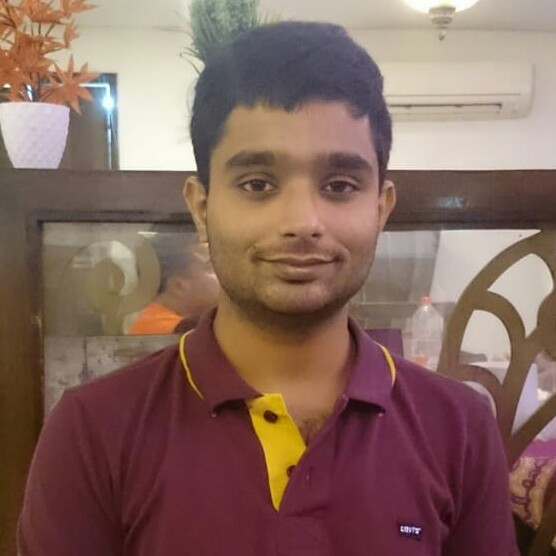
\includegraphics[width=1in,height=1.25in,clip,keepaspectratio]{../figures/photo_aryan.jpg}}]{Aryan Ritwajeet Jha}
	Aryan is pursuing his PhD in Electrical and Computer Engineering at the School of Electrical Engineering and Computer Science,  Voiland College of Engineering and Architecture, Washington State University, Pullman. His research interests are in Power Systems and High Voltage Engineering.
\end{IEEEbiography}

\printbibliography
\end{document}


